\chapter{酸碱平衡紊乱}

\section{前沿学术综述}

机体的组织细胞必须处于具有适宜酸碱度的体液环境中,才能进行正常的生命活动,细胞外液适宜的酸碱度用pH表示,正常值为7.35~7.45,是一个变动范围很窄的弱碱性环境。虽然机体在代谢过程中不断生成酸性或碱性物质,也经常摄取一些酸性或碱性食物,但依靠体液的缓冲系统以及肺和肾的调节作用,血浆pH稳定在正常范围,这种生理情况下维持体液酸碱度的相对稳定性称为酸碱平衡。

尽管机体对酸碱负荷具有强大的缓冲能力和有效的调节功能,但有许多原因可以引起酸碱负荷过量或调节机制障碍,导致体液酸碱度稳定性破坏,形成酸碱平衡紊乱。血pH低于7.35称为酸血症,碱血症则指血pH高于7.45。

危重患者的酸碱平衡紊乱尤为常见。很多疾病均可伴有酸碱平衡紊乱的发生,且一旦并发酸碱平衡紊乱则必将加速原发疾病的恶化,甚至导致死亡。临床工作中应十分重视对酸碱平衡紊乱的纠正,但是酸碱平衡紊乱的情况不同于某一种疾病的发生发展过程,某一种疾病尽管也可累及多个器官、系统,但其主要的病理改变仍限于某一器官和系统。酸碱平衡紊乱则不同,各个器官、系统的疾病均可导致酸碱平衡紊乱,机体所有细胞的功能代谢均参与其中,且多个器官组织立即参与代偿反应。这些决定了酸碱平衡紊乱时机体内出现极为复杂的病理生理改变。因此,在疾病的诊治中,往往需及时准确地判断体内发生的酸碱平衡紊乱情况,但解决这一问题并不简单
\protect\hyperlink{text00026.htmlux5cux23ch1-25}{\textsuperscript{{[}1{]}}}
。

一般来说,酸碱平衡紊乱的治疗首先应查找原因,针对原发疾病治疗,而不是急于把pH纠正到正常范围,因为盲目的治疗导致的后果可能比酸碱平衡紊乱本身更严重。充分考虑造成病理生理变化的原因,比纠正pH对患者更重要。如对于代谢性碱中毒的治疗应着重去除导致碱中毒的因素,纠正脱水的同时,及时纠正电解质紊乱。又如单纯性呼吸性酸中毒的治疗,主要是积极改善通气,控制感染,使原发性升高的二氧化碳分压下降,而不盲目补碱,特别是慢性呼吸性酸中毒更应慎重。对于代谢性酸中毒的治疗应积极治疗原发疾病,同时酌情补充碱性药物;对\ce{HCO3-}
低于10mmol/L的危重病患者应立即输液并使用碱剂治疗。

混合性酸碱平衡紊乱治疗的关键是正确认识、正确判断哪一种酸碱平衡紊乱是原发的,哪一种是代偿的,代偿的对机体是有利的,不宜纠正,否则会带来不良后果。此外,混合性酸碱平衡紊乱与水、电解质的关系非常密切,如脱水、低血氯、低血钾与碱中毒往往同步发生,应积极纠正。三重酸碱平衡紊乱的治疗,应首先掌握三重酸碱平衡紊乱的发生发展和演变规律,在治疗原发病的同时,应积极设法将三重酸碱平衡紊乱变为二重,争取尽快转变为单纯性酸碱平衡紊乱
\protect\hyperlink{text00026.htmlux5cux23ch2-25}{\textsuperscript{{[}2{]}}}
。

总之,危重患者内环境变化复杂,各种酸碱平衡紊乱可同时存在,其特点是发病率高、类型复杂、变化迅速和病死率高,且混合性酸碱平衡紊乱在临床工作中治疗较困难,对预后影响较大。因此监测动脉血气,正确地判断和处理,尽可能地控制酸碱紊乱的发生,对降低危重患者的死亡率有重要的临床意义。

\section{临床问题}

\subsection{酸碱的常用指标及临床意义}

\subsubsection{反映酸碱平衡紊乱的常用指标有哪些?临床意义是什么?}

目前常用的酸碱指标有:

(1)H\textsuperscript{+} 浓度和pH 血液的H\textsuperscript{+}
浓度很低,直接表示不方便,因此临床广泛使用H\textsuperscript{+}
浓度的负对数即pH表示。正常动脉血pH为7.35~7.45,血pH低于7.35称为酸血症,高于7.45称为碱血症。酸血症与碱血症不可能同时存在,但酸中毒与碱中毒可以同时存在,因此pH本身不能区分酸碱平衡紊乱的性质。

(2)动脉血二氧化碳分压 动脉血二氧化碳分压是指动脉血中呈物理状态溶解在血浆中的二氧化碳分子所产生的张力。因为二氧化碳弥散速度很快,动脉血二氧化碳分压与肺泡气二氧化碳分压近似,所以动脉血二氧化碳分压是反应呼吸性酸碱平衡紊乱的重要指标。动脉血二氧化碳分压正常值为35~45mmHg,平均40mmHg。动脉血二氧化碳分压增高表示肺泡通气不足,见于呼吸性酸中毒或代偿后的代谢性碱中毒;动脉血二氧化碳分压降低表示肺泡通气过度,见于呼吸性碱中毒或代偿后的代谢性酸中毒。

(3)标准碳酸氢盐(SB)和实际碳酸氢盐(AB) SB是指在标准条件下(38℃,血氧饱和度为100%,动脉血二氧化碳分压为40mmHg)所测得的血浆\ce{HCO3-}
含量,正常值为22~26mmol/L,平均24mmol/L。因为排除了呼吸因素的影响,故SB是反映代谢性酸碱平衡紊乱的指标,代谢性酸中毒时降低,代谢性碱中毒时升高。

AB是隔绝空气的标本在实际体温、动脉血二氧化碳分压和血氧饱和度条件下测得的血浆\ce{HCO3-}
含量。AB受呼吸和代谢两方面的影响。AB>SB表明有二氧化碳潴留,见于呼吸性酸中毒或代偿后的代谢性碱中毒;AB<SB表明过度通气,见于呼吸性碱中毒或代偿后的代谢性酸中毒。

(4)碱剩余(BE) BE是指在标准条件下,将1L全血或血浆的pH滴定到7.40时所需要的酸或碱的量,BE正常值为0±3mmol/L。代谢性酸中毒时,需用碱滴定,说明血液碱过少,BE用负值表示;代谢性碱中毒则相反。但在慢性呼吸性酸中毒或碱中毒时,BE亦可出现代偿性升高或降低。

(5)阴离子间隙(AG) AG是指血浆中未测定的阴离子与未测定的阳离子的差值。由于细胞外液阴阳离子总量相等,故AG可用血浆中可测定的阴离子与可测定的阳离子的差算出,正常值为10~14mmol/L。AG实质上是反映血浆中固定酸含量的指标,因此AG能够帮助区别代谢性酸中毒的类型和诊断混合性酸碱平衡紊乱。AG的计算公式为:

\[
\text{AG}=[\ce{Na+}]-[\ce{HCO3-}]-[\ce{Cl-}]    
\]

(6)二氧化碳结合力 指血浆中呈化学结合状态的二氧化碳的量。反映血浆中\ce{HCO3-}
的含量,正常值为23~31mmol/L。二氧化碳结合力增高可以是代谢性碱中毒或代偿后的呼吸性酸中毒;二氧化碳结合力降低可以是代谢性酸中毒或代偿后的呼吸性碱中毒。近年来随着血气分析仪的普及,二氧化碳结合力因其局限性而被取代。

\subsubsection{酸中毒可导致哪些病理生理变化?}

危重病患者的酸碱平衡紊乱非常常见。很多疾病均可伴有酸中毒的发生,酸中毒后的病理生理变化有:

(1)心血管系统 轻度的酸中毒导致交感神经兴奋而发生心动过速。严重酸中毒对心血管系统的直接作用是导致心动过缓。代谢性酸中毒降低心室纤颤阈值。呼吸因素导致酸中毒的影响不十分清楚,但很可能也是降低室颤阈值。

随pH的降低,心肌收缩力下降,增加细胞内的钙离子浓度能够拮抗这种作用。代谢性和呼吸性酸中毒对于心肌细胞的作用相似,但呼吸性酸中毒的作用更迅速,这是因为CO\textsubscript{2}
能够很快进入心肌细胞。

(2)神经肌肉 呼吸性酸中毒能够明显增加大脑的血流,动脉血二氧化碳分压迅速上升超过60mmHg时,会发生头痛;动脉血二氧化碳分压增加超过70mmHg时,会发生意识丧失和抽搐。这主要是因为细胞内pH降低而不是高CO\textsubscript{2}
的结果。事实上,慢性CO\textsubscript{2}
升高,如慢性阻塞性肺疾病患者能够耐受的动脉血二氧化碳分压可高达150mmHg。慢性呼吸衰竭急性发作时发生的肺性脑病的原理不十分清楚,但可能和细胞内酸中毒、低氧和神经内分泌等因素有关。因此说CO\textsubscript{2}
麻醉是CO\textsubscript{2} 的直接作用的结果是不恰当的。

急性高碳酸血症导致膈肌收缩力和收缩持续时间降低。慢性呼吸性酸中毒降低膈肌功能的作用还不明确。代谢性酸中毒对呼吸肌的影响尚不清楚。

(3)电解质 快速输注盐酸可导致血清钾升高。然而,在组织酸中毒如乳酸和酮症酸中毒时,血钾水平不但不高反而可能降低。在乳酸酸中毒和酮症酸中毒时低钾血症是普遍现象,较其他因素引起的低钾改变更明显。急性呼吸性酸中毒时血钾不变或仅轻度变化。呼吸性和代谢性酸中毒都会引起细胞外磷酸盐浓度升高。

\subsubsection{碱中毒的病理生理变化是什么?}

碱中毒后主要的病理生理变化有:

(1)心血管系统 碱血症至少要在pH达7.7时才表现出心肌收缩力增加。对室颤的阈值几乎没有影响。碱中毒患者发生房性或室性心律失常时,往往碱血症纠正后才易纠正。

体外实验中碱血症使外周血管扩张,pH
7.65时作用最强。临床上,过度通气可使血压和外周血管阻力降低。碱血症对血管的主要作用是血管扩张,但一些血管表现为收缩,特别是脑血管。碱血症也使冠状动脉痉挛并在心电图上出现明显变化。

(2)神经肌肉 急性呼吸性碱血症降低脑部血流,当动脉血二氧化碳分压降低到30mmHg时,脑血流下降到70%。动脉血二氧化碳分压在20mmHg时,脑血流下降最多,达基本血流的50%,但这种作用仅仅持续6小时。急性过度通气可以导致肌红蛋白代谢紊乱和意识改变。碱血症可以轻度增加呼吸肌收缩力。

(3)电解质 代谢性碱中毒导致钾离子下降和磷酸盐轻度下降,pH每下降0.1,钙离子下降0.03~0.09mmol/L。过度通气时常发生局部麻痹、腕痉挛、手足抽搐等,可能是氢离子对神经系统直接作用的结果。

(4)肺脏影响 碱血症导致呼吸衰竭患者的肺部分流增加,动脉血氧分压降低,这是由于通气/血流比例失调造成的。

(5)氧输送 碱血症增加血红蛋白与氧的结合力。临床上碱血症对氧输送的影响较小,但对存在组织缺氧的患者来说,血红蛋白与氧的亲和力增加是有害的。

\subsection{单纯性酸碱平衡紊乱}

\subsubsection{单纯性酸碱平衡紊乱的类型有哪些?}

单纯酸碱平衡紊乱的类型有:

(1)代谢性酸中毒 指细胞外液H\textsuperscript{+}
增加或\ce{HCO3-}
丢失而引起的,以原发性\ce{HCO3-}
降低为特征的酸碱平衡紊乱。

(2)代谢性碱中毒 指细胞外液碱增多或H\textsuperscript{+}
丢失而引起的,以原发性\ce{HCO3-}
浓度升高为特征的酸碱平衡紊乱。

(3)呼吸性酸中毒 二氧化碳排出障碍或二氧化碳吸入过多引起的,以原发性动脉血二氧化碳分压增加为特征的酸碱平衡紊乱。

(4)呼吸性碱中毒 肺过度通气引起的,以原发性动脉血二氧化碳分压降低为特征的酸碱平衡紊乱。

\subsubsection{什么是阴离子间隙?有什么临床意义?}

阴离子间隙是指血浆中未测定的阴离子与未测定的阳离子的差值。正常值为10~14mmol/L,阴离子间隙实质上是反映血浆中固定酸含量的指标,因此阴离子间隙能够帮助区别代谢性酸中毒的类型和诊断混合性酸碱平衡紊乱。阴离子间隙的计算公式为:

\[
\text{阴离子间隙}=[\ce{Na+}]-[\ce{HCO3-}]-[\ce{Cl-}]    
\]

代谢性酸中毒在病因学上分为阴离子间隙增加型和阴离子间隙正常型。阴离子间隙正常型酸中毒是因为\ce{HCO3-}
中和H\textsuperscript{+} 而丢失、Cl\textsuperscript{-}
浓度相应增加所致;阴离子间隙增加型代谢性酸中毒是因为未常规测量的阴离子取代了\ce{HCO3-}
。

(1)阴离子间隙正常型酸中毒 阴离子间隙正常型酸中毒的特点是各种原因引起血浆中的\ce{HCO3-}
浓度降低,同时伴有血Cl\textsuperscript{-}
代偿性增高。常见原因:①消化道丢失\ce{HCO3-}
。肠液、胰液和胆汁中\ce{HCO3-}
的含量高于血浆,在腹泻、肠瘘和胆瘘的患者,可因\ce{HCO3-}
大量丢失,而使血浆中\ce{HCO3-}
减少,从而肾小管H\textsuperscript{+} -Na\textsuperscript{+}
交换减少,Na\textsuperscript{+} 与Cl\textsuperscript{-}
重吸收增多,致血Cl\textsuperscript{-}
浓度升高。②含氯酸性药物摄入过多。长期或大量使用氯化铵、盐酸精氨酸等含氯酸性药物,此类药物在代谢过程中可产生H\textsuperscript{+}
和Cl\textsuperscript{-} ,Cl\textsuperscript{-}
增多促使近曲小管重吸收NaCl增加,远曲小管内Na\textsuperscript{+}
含量减少,H\textsuperscript{+} -Na\textsuperscript{+}
交换减少,\ce{HCO3-}
重吸收减少;此外,大量输入生理盐水可因其中的Cl\textsuperscript{-}
含量高于血浆,而引起阴离子间隙正常型代谢性酸中毒。③肾脏泌H\textsuperscript{+}
功能障碍。肾功能减退但尚未出现\ce{HPO4^2-}
、\ce{SO4^2-}   
等阴离子潴留,可因肾小管泌H\textsuperscript{+}
和重吸收\ce{HCO3-}
减少而引起阴离子间隙正常型酸中毒;肾小管酸中毒,近端肾小管酸中毒是由于近曲小管重吸收\ce{HCO3-}
减少,远端肾小管酸中毒是由于远曲小管泌H\textsuperscript{+}
障碍,H\textsuperscript{+}
在体内潴留,血浆\ce{HCO3-}
浓度降低;还有应用碳酸酐酶抑制剂如乙酰唑胺抑制肾小管上皮细胞内碳酸酐酶活性,使碳酸产生减少,泌H\textsuperscript{+}
和重吸收\ce{HCO3-} 减少。

(2)阴离子间隙增高型酸中毒 阴离子间隙增高型酸中毒的特点是阴离子间隙增高,但血Cl\textsuperscript{-}
正常,其原因包括:①固定酸摄入过多。如过量服用水杨酸类药物,使血浆中的有机酸阴离子增加。②固定酸产生过多。常见的有乳酸酸中毒及酮症酸中毒,乳酸酸中毒是各种原因引起的组织低灌注或缺氧导致乳酸产生增加;酮症酸中毒指严重饥饿、酒精中毒等情况时,葡萄糖利用减少或糖原储备不足,脂肪分解加速,产生大量酮体,当酮体的产生量超过外周组织的氧化能力及肾排泄能力时,可能发生酮症酸中毒。③肾排泄固定酸减少。急(慢)性肾衰竭时致肾小球滤过率低于正常值的25%时,机体代谢产生的\ce{HPO4^2-}
、\ce{SO4^2-}
等不能充分排出,使血中固定酸增加。

\subsubsection{乳酸的临床意义是什么?}

动脉血乳酸的正常值为1~1.5mmol/L。该值超过2mmol/L应引起临床医生的高度重视;若动脉血乳酸水平超过4mmol/L,同时动脉血pH低于7.35,则诊断为乳酸酸中毒。休克患者组织灌注不足可引起无氧代谢、乳酸产生增多,是导致乳酸酸中毒的主要原因。乳酸酸中毒是危重患者常见的代谢性酸中毒,动脉血乳酸水平增高,提示组织缺氧,因此监测乳酸变化的水平有助于估计休克的复苏效果和变化趋势。

乳酸的价值不仅是反映机体缺氧严重程度,更为重要的是可以间接反映各个脏器功能衰竭的严重程度,临床上发现随着多器官功能衰竭评分逐渐增高,机体乳酸值相应增高,病死率亦相应增加。

如果动态监测乳酸并观察乳酸随时间变化关系,可以帮助临床医生及时发现病情变化:当乳酸有逐渐下降趋势,提示干预治疗可能有效,病情趋于好转;相反,当血乳酸持续增高或者在治疗中乳酸水平突然增高,则提示病情恶化,乳酸急剧增高,多属于临终前变化。

Tuchschmidt等比较各种原因休克患者动脉血乳酸、血流动力学指标发现,与急性生理和慢性健康状况评分(APACHEⅡ评分)相比,乳酸预测患者预后的准确性较高,且乳酸水平能在一定程度上反映疾病的严重程度。

虽然乳酸水平能在一定程度上反映疾病的严重程度,但因为乳酸受某些因素如营养状态和肝脏疾病的影响,故而仅凭乳酸水平做出预后判断是片面的。但乳酸水平改变的趋势有助于评定治疗效果和判断预后
\protect\hyperlink{text00026.htmlux5cux23ch3-25}{\textsuperscript{{[}3{]}}}
。

\subsubsection{乳酸酸中毒的常见病因是什么?该如何处理?}

(1)乳酸酸中毒的病因

缺血缺氧低灌注:组织细胞灌注不良必然导致细胞缺氧,进行无氧代谢而致乳酸产生增加,此为乳酸酸中毒最常见的原因,也是乳酸增高的经典机制。

严重全身感染:严重全身感染是引起重症医学科患者乳酸酸中毒的最常见原因。严重全身感染引起乳酸酸中毒的原因仍不清楚,有几种导致乳酸水平增高的发病机制假说:①虽然经过积极的复苏治疗,患者仍然组织缺氧、微循环功能障碍,存在无氧代谢,导致乳酸酸中毒;②高分解代谢状态使丙氨酸、丙酮酸和乳酸同比例增加;③局部组织低氧而使乳酸产生增加、导致乳酸酸中毒。

癫痫发作:癫痫大发作导致肌肉能量储备和肝糖原耗竭,许多葡萄糖转变为乳酸。发作时乳酸水平经常超过10mmol/L,pH低于7.20。

恶性肿瘤:据报道,有多种恶性肿瘤可发生乳酸酸中毒,最常见的是白血病和淋巴瘤。乳酸盐产生增多的机制与氧化磷酸化和糖酵解异常有关。当然,恶性肿瘤患者的乳酸酸中毒大都发生在患者休克或严重全身感染时。

肝衰竭:肝脏是重要的乳酸代谢器官,严重肝脏疾病时,乳酸清除减慢。对于稳定的慢性肝脏疾病患者,即使存在严重的肝脏功能障碍也不会明显增加血浆乳酸水平。对于爆发性肝衰竭患者,因为乳酸盐清除严重障碍而使患者表现为乳酸酸中毒。

其他原因:氰化物、酒精(乙醇)或甲醇中毒、先天性1,6-二磷酸果糖缺乏等原因,也会导致乳酸酸中毒。

(2)治疗 首先应病因治疗,对症治疗的目的在于避免乳酸酸中毒本身对机体造成的损害进一步加重。对症治疗的方法包括:①补充碳酸氢盐,虽然对碳酸氢盐的安全性和有效性至今仍有不同观点,但仍长期以来被用作治疗乳酸酸中毒的标准治疗方法。碳酸氢盐治疗的目的在于减轻酸血症对血流动力学的影响。但碳酸氢盐治疗可能使动脉血二氧化碳分压增高从而引起细胞内pH迅速降低;②透析,血液透析和腹膜透析都可用来治疗乳酸酸中毒。碳酸氢盐或醋酸盐都可以作为缓冲液应用于透析
\protect\hyperlink{text00026.htmlux5cux23ch4-25}{\textsuperscript{{[}4{]}}}
。当然,血流动力学不稳定的患者,应采用连续肾脏替代治疗。

\subsubsection{什么是酮症酸中毒?只有糖尿病能引起酮症酸中毒吗?}

酮症酸中毒发生在游离脂肪酸产生增加或脂肪酸分解的酮体在肝脏内蓄积的情况下。除糖尿病酮症酸中毒外,还有饥饿性酮症和酒精性酮症,但糖尿病酮症酸中毒最常见,可以通过病史、血糖水平和酮体加以鉴别。

酒精性酮症酸中毒发生在大量饮酒后反复呕吐者,表现为血酮体增高的同时血糖正常或轻度增高的特点。饥饿性酮症酸中毒是轻微和有自限性的酸中毒,\ce{HCO3-}
的降低很少超过5mmol/L,合并糖尿病酮症酸中毒应通过静脉应用胰岛素治疗,补充碳酸氢盐治疗糖尿病酮症酸中毒无效。对于绝大部分的酒精性酮症酸中毒患者来说,既不需要碳酸氢盐也不需要胰岛素治疗,对输注葡萄糖反应灵敏。饥饿性酮症酸中毒予以进食能迅速纠正。

\subsubsection{如何鉴别糖尿病性酮症酸中毒与糖尿病性高渗高血糖昏迷?}

酮症酸中毒和高渗性昏迷是糖尿病的两个最严重的急性并发症,即使在正规治疗中也可能发生。这些急症可发生在Ⅰ型和Ⅱ型糖尿病患者。糖尿病酮症酸中毒死亡率不到5%,高渗性高血糖状态的死亡率则高达15%。高龄患者和儿童或合并昏迷、低血压者预后更差。

糖尿病酮症酸中毒与高渗性高血糖状态患者两种代谢紊乱的发病机制基本是一致的,就是血中胰岛素有效作用的减弱,同时多种升血糖激素水平升高,如胰高血糖素、儿茶酚胺、糖皮质激素、生长激素等。糖尿病酮症酸中毒与高渗性高血糖状态患者由于这些激素水平的变化而导致肝及肾脏葡萄糖生成增加、外周组织对葡萄糖的利用降低,导致高血糖,同时细胞外液渗透压升高。糖尿病酮症酸中毒时,由于胰岛素作用减弱以及升糖激素作用增强,共同使脂肪组织分解为游离脂肪酸,释放入血液循环,在肝脏氧化分解产生酮体,从而造成酮血症及代谢性酸中毒。高渗性高血糖状态虽然由于血浆胰岛素水平不足,胰岛素敏感组织不能有效利用葡萄糖,但有学者推测患者体内尚有一定量的胰岛素可以抑制脂肪组织分解,并不产生酮体。糖尿病酮症酸中毒和高渗性高血糖状态均能造成尿糖增高引起渗透性利尿,从而使机体脱水,失钠、钾和其他电解质成分。

糖尿病酮症酸中毒和高渗性高血糖状态的典型临床表现及实验室检查见表\ref{tab20-1}。

\begin{table}[htbp]
\centering
\caption{糖尿病酮症酸中毒(DKA)和高渗性高血糖状态(HHS)典型临床表现及实验室检查}
\label{tab20-1}
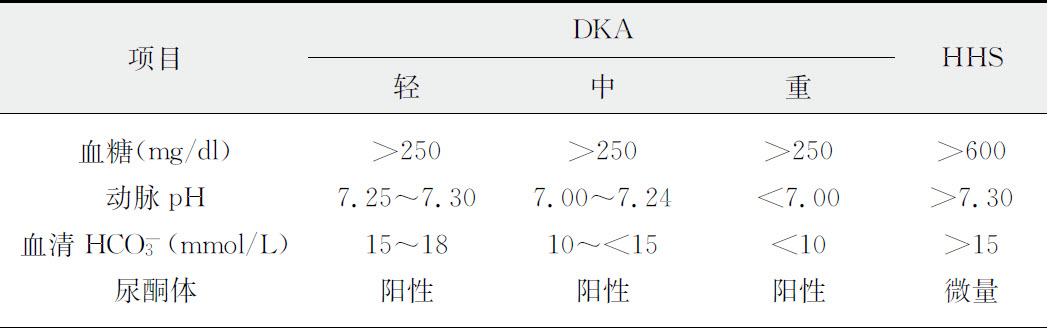
\includegraphics{./images/Image00197.jpg}
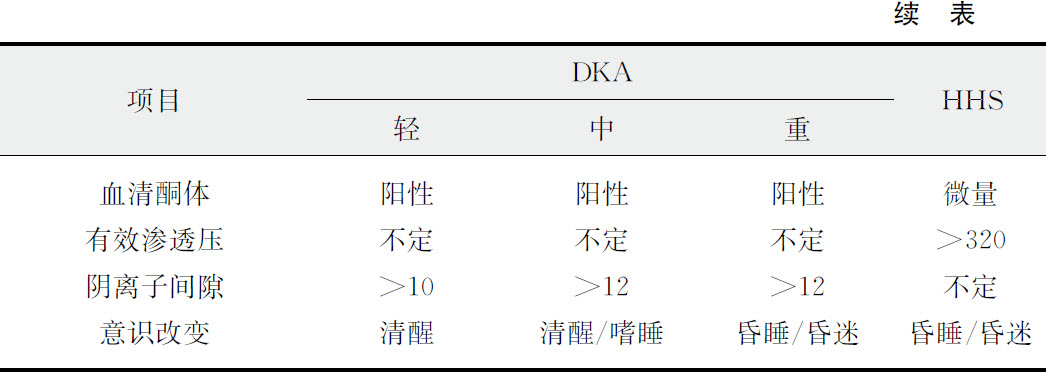
\includegraphics{./images/Image00198.jpg}
\end{table}

高渗性高血糖状态发病缓慢,历经数日到数周,而1型、甚至2型糖尿病导致的糖尿病酮症酸中毒常呈急性发病。尽管糖尿病控制不良的症状可存在数天,但酮症酸中毒的代谢改变在短时间形成(一般<24小时)。有时全部症状可骤然发生,事先无任何先兆或症状。糖尿病酮症酸中毒和高渗性高血糖状态的临床表现均可有多尿、多饮、多食、体重减少、呕吐、腹痛(仅糖尿病酮症酸中毒)、脱水、虚弱无力、意识模糊、最终陷入昏迷;体格检查可有皮肤弹性差、Kussmaul呼吸(仅糖尿病酮症酸中毒)、心动过速、低血压、精神改变、最终昏迷(更常见于高渗性高血糖状态)。25%的糖尿病酮症酸中毒患者表现呕吐,并可能呕吐咖啡样物,潜血阳性,胃镜检查证实为出血性胃炎。患者的神志改变可从完全清醒到昏睡、昏迷,高渗性高血糖状态更常出现昏睡、昏迷。尽管感染是糖尿病酮症酸中毒和高渗性高血糖状态的常见诱因,但由于早期外周血管舒张,患者可体温正常,甚至低体温。患者出现低体温是预后不良的标志。对腹痛患者需小心谨慎,因为腹痛既可以是糖尿病酮症酸中毒的结果,也可能是糖尿病酮症酸中毒的诱因(尤其在年轻患者)。如果脱水或代谢性酸中毒纠正后腹痛仍不缓解,则需进一步检查以明确诊断。

\subsubsection{怎样鉴别糖尿病酮症酸中毒和糖尿病乳酸酸中毒?}

糖尿病患者易发生酮症酸中毒和糖尿病乳酸酸中毒,由于很多医院不能测定血乳酸,故乳酸酸中毒易被忽视。糖尿病酮症酸中毒通常经补液、补碱、胰岛素治疗有效,病死率<1%,而乳酸酸中毒病死率高达50%以上,老年患者病死率更高,可达80%以上,故应重视糖尿病患者是否发生乳酸酸中毒。

临床诊断乳酸酸中毒要点如下:①有口服双胍类降糖药物史,尤其是苯乙双胍。②动脉血乳酸>1.5mmol/l(正常动脉血乳酸范围为1~1.5mmol/L)。③体液碱贮备减少,阴离子间隙>18mmol/L(正常范围8~16mmol/L,平均12mmol/L)。④代谢性酸中毒,血pH<7.35。在以上4个指标中,诊断乳酸酸中毒最重要的是血乳酸水平的升高,动脉血的pH及阴离子间隙是两个相对不敏感的指标。高乳酸血症可呈酸血症、正常血pH或碱血症,主要取决于血乳酸增高程度、体液缓冲能力以及是否合并其他疾病,如败血症、肝、肾、心脏等脏器功能障碍或功能衰竭。临床如没有条件测定血乳酸水平,也可根据阴离子间隙计算推测,阴离子间隙增大的常见原因有:糖尿病或酒精性酮症酸中毒、尿毒症性酸中毒、乳酸酸中毒、化学毒素摄取后酸中毒(如误服大量水杨酸、甲醇、乙二醛、副醛)。如无尿毒症又无酮症酸中毒,也无其他原因可解释的酸中毒,则阴离子间隙则显著增大常提示乳酸酸中毒。

糖尿病酮症酸中毒的临床特点为起病较缓,症状、体征、实验室检查与乳酸酸中毒相似,但血乳酸在糖尿病酮症酸中毒时正常、乳酸酸中毒时明显增高,单纯的糖尿病酮症酸中毒血乳酸基本正常。

\subsubsection{糖尿病酮症酸中毒该如何补碱?}

糖尿病酮症酸中毒患者中,轻症患者经补液合注射胰岛素后,酸中毒可逐渐纠正,不必补碱。当血pH低至7.0时,有抑制呼吸中枢和中枢神经功能、诱发心律失常的危险,故应给予相应治疗。但补充碳酸氢钠过多过快又可产生不利的影响。如血pH降至7.1,或\ce{HCO3-}
降至5mmol/L(相当于二氧化碳结合力4.5~6.7mmol/L),应给予碳酸氢钠50mmol/L,可用5%的碳酸氢钠84ml,用注射用水稀释成1.25%溶液,静脉滴注。如血pH>7.1或\ce{HCO3-}
>10mmol/L(相当于二氧化碳结合力11.2~13.5mmol/L),无明显酸中毒大呼吸者,可暂不予补碱。在纠正代谢紊乱过程中,代谢性酸中毒也会得到改善和纠正。

糖尿病酮症酸中毒的补碱治疗中,碳酸氢盐的使用仍有争议。美国糖尿病学会推荐:若pH<6.9,可将100mmol碳酸氢盐加入到400ml注射用水中以200ml/小时的速度静脉滴入;若pH介于6.9~7.0之间,经前瞻性随机研究未能证实使用碳酸氢盐能降低致残率及病死率,但考虑到严重的酸中毒会导致严重的心血管副作用,成人患者慎重地使用碳酸氢盐是可取的。可将50mmol碳酸氢盐加入到200ml注射用水中以200ml/小时的速度静脉滴入;每2小时检测静脉血pH,直至pH升至7.0;如果有必要,应该每2小时重复补碱。若pH>7.0,可暂不使用碳酸氢盐,但应积极补液和使用胰岛素,阻止脂肪分解。

另外,碳酸氢钠和胰岛素治疗均可降低血钾浓度,因此,在补液治疗过程中一定要坚持补钾并严密监测血钾浓度。

\subsubsection{代谢性碱中毒的常见病因有哪些?}

凡是引起H\textsuperscript{+}
丢失或\ce{HCO3-}
进入细胞外液增多的因素,都可以引起血浆\ce{HCO3-}
浓度升高。正常情况下,肾脏可减少\ce{HCO3-}
重吸收,维持血浆正常\ce{HCO3-}
浓度,以避免代谢性碱中毒发生。但在某些情况下,如有效循环血量不足、低氯等,造成肾脏对\ce{HCO3-}
的调节功能障碍,使血浆\ce{HCO3-}
水平升高,可发生代谢性碱中毒。

(1)消化道丢失H\textsuperscript{+}
 见于频繁呕吐以及胃肠减压,富含H\textsuperscript{+}
的胃液大量丢失后,肠液中的\ce{HCO3-}
得不到中和而被吸收入血,以致血浆中\ce{HCO3-}
浓度升高,发生代谢性碱中毒。

(2)肾丢失H\textsuperscript{+}
 ①低氯性碱中毒:噻嗪类和袢利尿剂通过抑制髓袢升支对Cl\textsuperscript{-}
的主动重吸收,使Na\textsuperscript{+}
的被动重吸收减少,远曲小管液中的NaCl含量增高,H\textsuperscript{+}
-Na\textsuperscript{+} 、K\textsuperscript{+} -Na\textsuperscript{+}
交换增加,Cl\textsuperscript{-}
以氯化铵的形式排出,H\textsuperscript{+} -Na\textsuperscript{+}
交换增加使\ce{HCO3-}
重吸收增加,引起低氯性碱中毒。②肾上腺皮质激素增多:肾上腺皮质激素增多促使肾远曲小管和集合管H\textsuperscript{+}
-Na\textsuperscript{+} 、K\textsuperscript{+} -Na\textsuperscript{+}
交换增加,\ce{HCO3-}
重吸收增加,导致代谢性碱中毒和低钾血症,后者又促进碱中毒的发展。

(3)H\textsuperscript{+}
向细胞内转移 低钾血症时,细胞内钾向细胞外转移以代偿血钾降低,作为交换,细胞外液中的H\textsuperscript{+}
移入细胞内,造成细胞外碱中毒和细胞内酸中毒。同时,因肾小管上皮细胞缺钾,K\textsuperscript{+}
-Na\textsuperscript{+} 交换减少H\textsuperscript{+}
-Na\textsuperscript{+} 交换增加,H\textsuperscript{+}
排出增加,\ce{HCO3-}
重吸收增加,造成低钾性碱中毒。

(4)碱性物质摄入过多 口服或静脉输入碳酸氢盐过量可引起代谢性碱中毒。大量输入库存血,库血中的枸橼酸钠在体内氧化产生碳酸氢钠,在肾功能减退时可引起代谢性碱中毒。

\subsubsection{如何纠正代谢性碱中毒?}

代谢性碱中毒一般是可以预防的。如果发生代谢性碱中毒,一般纠正电解质紊乱能恢复酸碱平衡。与氯化物不足有关的必须补充足量的氯化物。

常用的纠正代谢性碱中毒方法,包括盐酸精氨酸、氯化铵和盐酸。近来有学者认为盐酸精氨酸和氯化铵可能会潜在增加细胞内pH,因此不提倡使用。

应用浓度在100~200mmol/L的盐酸治疗代谢性碱中毒是安全的,根据碱中毒的严重程度和它的影响程度,输注速度在20~50mmol/小时,但必须通过中心静脉输注,必须每小时监测动脉血pH。

\subsubsection{如何区分急性呼吸性酸中毒和慢性呼吸性酸中毒?}

呼吸性酸中毒是二氧化碳排出障碍或二氧化碳吸入过多引起的,以原发性动脉血二氧化碳分压增加为特征的酸碱平衡紊乱。依照发病速度和病程长短分为急性呼吸性酸中毒和慢性呼吸性酸中毒。急性呼吸性酸中毒常见于急性气道堵塞、急性心源性肺水肿、中枢或呼吸肌麻痹引起的呼吸骤停及急性呼吸窘迫综合征等。慢性呼吸性酸中毒常见于气道及肺部慢性炎症引起的慢性阻塞性肺疾病、肺广泛性纤维化或肺不张,一般指动脉血二氧化碳分压高浓度潴留达24小时以上者。

急性呼吸性酸中毒时,由于肾脏的代偿功能十分缓慢,因此仅主要靠细胞内外离子交换及细胞内缓冲,这种调节与代偿十分有限,常表现为代偿不足或失代偿状态。动脉血二氧化碳分压每升高10mmHg,血浆\ce{HCO3-}
仅升高0.7~1mmol/L,不足以维持\ce{HCO3-}
/H\textsubscript{2} CO\textsubscript{3}
的正常比值,所以急性呼吸衰竭酸中毒时pH往往低于正常值,呈失代偿状态。

慢性呼吸性酸中毒时,由于肾脏的代偿,有可能是代偿性的。慢性呼吸性酸中毒时由于动脉血二氧化碳分压和H\textsuperscript{+}
浓度升高,可能增强肾小管上皮细胞内碳酸酐酶和线粒体中谷胺酰胺酶活性,促使小管上皮排泌H\textsuperscript{+}
和泌NH\textsubscript{3} ·NH\textsubscript{4} \textsuperscript{+}
,同时增加对\ce{HCO3-}
的重吸收。这种作用的充分发挥常需3~5天才能完成,因此急性呼吸衰竭酸中毒来不及代偿,而在慢性呼吸性酸中毒时,由于肾脏的保碱作用较强大,而且随动脉血二氧化碳分压升高,\ce{HCO3-}
也呈比例增高,大致动脉血二氧化碳分压每升高10mmHg,血浆\ce{HCO3-}
增高3.5~4.5mmol/L,能使\ce{HCO3-}
/H\textsubscript{2} CO\textsubscript{3}
比值接近20∶1,因而在轻度和中度呼吸性酸中毒时有可能代偿。\ce{HCO3-}
继发性代偿升高最大的代偿时间为3~5天,代偿的限度为45mmol/L。

\subsubsection{呼吸性酸中毒的常见病因是什么?}

呼吸性酸中毒的常见病因有:

(1)呼吸中枢抑制 见于颅脑损伤、脑炎、脑血管意外、麻醉药或镇静药过量等,呼吸中枢抑制使肺泡通气量减少,引起二氧化碳潴留。

(2)呼吸肌麻痹 急性脊髓灰质炎、重症肌无力和脊髓高位损伤的患者,因呼吸动力不足而导致二氧化碳排出减少。

(3)呼吸道阻塞 见于喉头痉挛或水肿、异物阻塞气道等,呼吸道严重阻塞引起急性二氧化碳潴留。

(4)胸部疾病 胸部创伤、气胸、大量胸腔积液或胸廓畸形时,胸廓活动受限导致二氧化碳排出减少。

(5)肺部疾病 严重肺炎、慢性阻塞性肺疾病、哮喘或ARDS等广泛肺组织病变时,肺泡通气量减少,二氧化碳排出障碍。

(6)呼吸机使用不当 呼吸机通气量设置过小,使二氧化碳排出减少。

此外在通气不良的环境中二氧化碳浓度增加,从而吸入增多也可导致为呼吸性酸中毒。

\subsection{混合型酸碱平衡紊乱}

\subsubsection{混合型酸碱紊乱有哪些类型?}

混合型酸碱紊乱是指同一患者有两种或两种以上的单纯型酸碱平衡紊乱同时存在。如果代谢性和呼吸性异常均为酸中毒或碱中毒,称为相加性混合型酸碱平衡紊乱;如果代谢性和呼吸性异常呈相反方向变化,称为相消性混合型酸碱平衡紊乱(表\ref{tab20-2})\footnote{*呼酸:呼吸性酸中毒;呼碱:呼吸性碱中毒;代酸:代谢性酸中毒;代碱:代谢性碱中毒。}。因为同一患者不可能同时发生二氧化碳潴留和排出过多,因此呼吸性酸中毒和呼吸性碱中毒不可能同时存在。诊断混合型酸碱平衡紊乱必须在充分了解原发病及病情变化的基础上,结合实验室检查,从原发病入手,进行综合分析。

\begin{table}[htbp]
\centering
\caption{混合型酸碱平衡紊乱类型\textsuperscript{*}}
\label{tab20-2}
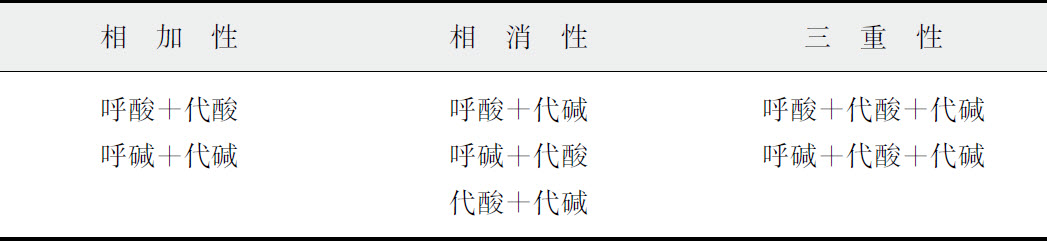
\includegraphics{./images/Image00219.jpg}
\end{table}



\subsubsection{如何诊断酸碱平衡紊乱?}

酸碱平衡紊乱的诊断是非常复杂的。许多重症患者存在多重紊乱。实验室检查包括pH,二氧化碳分压,碳酸氢盐水平,电解质水平等。

(1)首先要明确目前是酸血症还是碱血症 明确pH是低于7.35还是高于7.45。混合性紊乱时也许pH在正常范围,但碳酸氢盐、二氧化碳分压、阴离子间隙的改变都标志着酸碱平衡紊乱。

(2)明确主要紊乱是因为呼吸因素还是代谢因素引起的 对于酸血症,动脉血二氧化碳分压高于45mmHg说明为呼吸性酸中毒,碳酸氢盐水平低于22mmol/L意味着代谢性碱中毒。对于碱血症,动脉血二氧化碳分压低于35mmHg,提示呼吸性碱中毒,碳酸氢盐浓度大于26mmol/L说明为代谢性碱中毒。

(3)明确对于主要的紊乱来说是否发生了适当的代偿 代谢性紊乱伴有可以估计的与之相适应的呼吸代偿;呼吸性紊乱时碳酸氢盐浓度的变化分为两部分,急性变化是因为组织缓冲作用,慢性变化是由于肾脏的代偿性变化。呼吸性和代谢性紊乱的代偿预计值可用公式计算(表\ref{tab20-3})\footnote{* 当\ce{HCO3-}
>40mmol/L时,用公式$\text{PaCO}_2=0.75\times \ce{HCO3-}+19\pm 7.5$}。如果不在代偿预计值范围内,则可能有多重的酸碱紊乱。

\begin{table}[htbp]
\centering
\caption{单纯酸碱紊乱的代偿公式}
\label{tab20-3}
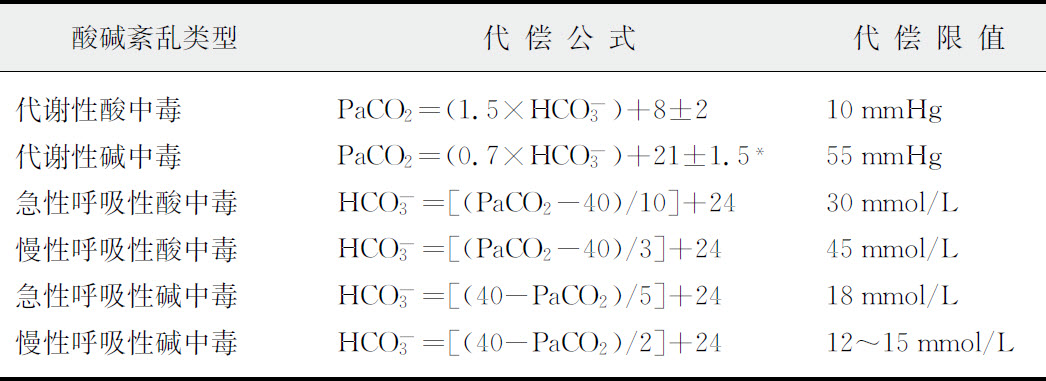
\includegraphics{./images/Image00220.jpg}
\end{table}



(4)计算阴离子间隙 阴离子间隙是指未测定的阴离子和未测定的阳离子之间的差值,用来判断代谢性酸中毒。未检测的阴离子一般指血浆蛋白,主要是白蛋白,其余为磷酸盐、硫酸盐等其他有机阴离子。阴离子间隙增高并不总意味着代谢性酸中毒,碱血症时阴离子间隙也会增加,因为这时血浆蛋白携带的净负电荷浓度增加。利尿也会增加阴离子间隙,因为蛋白浓度增加。但是,当阴离子间隙增高超过20mmol/L时,应考虑有代谢性酸中毒存在。

诊断和鉴别诊断酸碱平衡紊乱当然必须依赖具体患者的具体临床情况
\protect\hyperlink{text00026.htmlux5cux23ch5-25}{\textsuperscript{{[}5{]}}}
\textsuperscript{,}
\protect\hyperlink{text00026.htmlux5cux23ch6-25}{\textsuperscript{{[}6{]}}}
。

\subsubsection{慢性阻塞性肺疾病常见的混合性酸碱紊乱有哪些?}

(1)呼吸性酸中毒合并代谢性碱中毒 是慢性阻塞性肺疾病患者最常见的混合性酸碱失衡类型。常见原因有:①在通气未改善之前滥用NaHCO\textsubscript{3}
;②过急的过度人工通气;③大量使用利尿剂之后;④电解质紊乱。其特点为:动脉血二氧化碳分压和血浆\ce{HCO3-}
浓度均升高而且升高的浓度均已超出彼此正常代偿范围,血气中实际碳酸氢盐、标准碳酸氢盐和缓冲碱均升高,碱剩余正值加大,pH变化不大,略偏高或偏低,也可以在正常范围内。

呼吸性酸中毒合并代谢性碱中毒对机体危害性较大,病死率较高,原因在于:①呼吸抑制;②氧离曲线左移造成组织缺氧;③血清钙离子降低;④可造成消化道出血。此类失衡以医源性因素引起者较多,故应强调预防为主,避免过度通气,正确使用利尿剂,应采用排钾与保钾利尿剂联合应用,应间歇、短程,避免长期使用激素,严格掌握补碱指征。发生呼吸性酸中毒合并代谢性碱中毒时应给予补充氯化钾,根据病情轻重选择给药途径及剂量。低钙抽搐可使用氯化钙治疗,对于严重的低氯性碱中毒可选用盐酸精氨酸,但不宜大量或长期使用,以免造成高氯性代酸。

(2)慢性阻塞性肺疾病患者也会出现呼吸性酸中毒合并代谢性酸中毒,此类患者病情较严重,往往存在严重感染、呼吸衰竭及心力衰竭,因患者通气功能障碍导致二氧化碳排出受阻,同时由于严重感染缺氧,导致无氧代谢增加,造成乳酸堆积,并且可能存在潜在性肾功能不全而使体内酸性代谢产物排出受阻,或合并糖尿病及极度厌食、营养不足等造成酮症酸中毒。其特点为:由于呼吸性和代谢性因素指标均朝酸性反面变化,因此\ce{HCO3-}
减少时呼吸不能代偿,在动脉血二氧化碳分压增多时,肾脏也不能代偿\ce{HCO3-}
反而减少,两者不能互相代偿,呈严重失代偿状态,pH明显减低,并形成恶性循环,有致死性后果,患者血气中实际碳酸氢盐、标准碳酸氢盐和缓冲碱均降低,实际碳酸氢盐>标准碳酸氢盐,血浆钾离子浓度升高,阴离子间隙可增大。该类型的防治应首先针对病因、诱因和并发症进行治疗,一定要同时处理两种失衡,如抗感染、保持呼吸道通畅、减少死腔、增加肺泡通气量。适时使用呼吸兴奋剂或机械呼吸,严重缺氧引起乳酸酸中毒者,应在血气监测下适当提高吸氧浓度维持血氧饱和度、输注红细胞和增加心排血量,以增加全身氧供,纠正缺氧。

\begin{center}\rule{0.5\linewidth}{\linethickness}\end{center}

参考文献

\protect\hyperlink{text00026.htmlux5cux23ch1-25-back}{{[}1{]}}
.Benjamin E,Oropello JM,Abalos AM,et al.Effects of acid-base
correction on hemodynamics,oxygen dynamics,and resuscitability in
severe canine hemorrhagic shock.Crit Care Med,1994,22:1616-1620.

\protect\hyperlink{text00026.htmlux5cux23ch2-25-back}{{[}2{]}}
.Cardenas VJ,Zwischenberger JB,Tao W,et al.Correction of blood pH
attenuates changes in hemodynamics and organ blood flow during
permissive hypercapnia.Crit Care Med,1996,24:827-834.

\protect\hyperlink{text00026.htmlux5cux23ch3-25-back}{{[}3{]}}
.Stacpoole PW,Wright EC,Baumgartner TG,et al.Natural history and
course of acquired lactic acidosis in adults.Am J
Med,1994,97:47-52.

\protect\hyperlink{text00026.htmlux5cux23ch4-25-back}{{[}4{]}}
.Stacpoole PW,Wright EC,Baumgartner TG,et al.A controlled clinical
trial of dichloroacetate for treatment of lactic acidosis in adults.N
Engl J Med,1992,327:1564-1570.

\protect\hyperlink{text00026.htmlux5cux23ch5-25-back}{{[}5{]}} .Horacio
JA,Nicolaos EM.Management of life-threatening acid-base disorders.N
Engl J Med,1998,338:26-34.

\protect\hyperlink{text00026.htmlux5cux23ch6-25-back}{{[}6{]}} .Horacio
JA,Nicolaos EM.Management of life-threatening acid-base disorders.N
Engl J Med,1998,338:107-111.

\protect\hypertarget{text00027.html}{}{}

